\chapter{Introduzione}

\section{Calcolo parallelo}

Il calcolo parallelo è un paradigma di programmazione che consente di eseguire più operazioni contemporaneamente, sfruttando la potenza di elaborazione di più unità di calcolo. A differenza dello pseudoparallelismo, che simula l'esecuzione simultanea di più processi su un singolo processore, il calcolo parallelo utilizza effettivamente più processori o core per eseguire compiti in parallelo. 

Questo paradigma è utile perché riduce i tempi di esecuzione e aumenta la dimensione dei dati processabili, consentendo di affrontare problemi più complessi e di ottenere risultati più rapidamente. 

\section{Limiti del calcolo parallelo}

\subsection{Caso ideale di parallelizzazione}
Per comprendere i limiti del calcolo parallelo è utile partire da un modello ideale. 
Supponiamo che un programma sia completamente parallelizzabile, cioè che tutto il lavoro possa essere suddiviso tra più unità di calcolo senza alcuna parte sequenziale.

Se $T_0$ indica il tempo di esecuzione del programma in modalità sequenziale e $N$ il numero di unità di calcolo disponibili, il tempo di esecuzione ideale del programma parallelo sarebbe:

\[
T_L(N) = \frac{T_0}{N}
\]

In questo caso il tempo di esecuzione diminuisce linearmente all'aumentare del numero di processori. 
Lo speed-up ottenuto è quindi:

\[
S_L(N) = \frac{T_0}{T_L(N)} = N
\]

Questo significa che, in condizioni ideali, raddoppiare il numero di unità di calcolo dimezza il tempo di esecuzione. 
In tale modello non esiste quindi un limite teorico allo speed-up ottenibile aumentando il numero di processori.

\subsection{Legge di Amdahl}
Il calcolo parallelo non può essere applicato a tutti i problemi, e anche quando è possibile, esiste un limite alla velocità di esecuzione che può essere raggiunta. Questo limite è descritto dalla legge di Amdahl:

\begin{quote}
\textit{La velocità massima di un programma parallelo è limitata dalla frazione di codice che deve essere eseguita in modo sequenziale.}
\end{quote}
Adamahl ha dimostrato che se una frazione $p$ del programma può essere parallelizzata, allora la velocità massima teorica che si può ottenere è data da:
\[
T_A(N) = \frac{p T_0}{N} + (1-p) T_0
\]
dove $T_0$ è il tempo di esecuzione del programma sequenziale e $N$ è il numero di processori. Si può anche esprimere il massimo speed-up come:
\[
S_A(N) = \frac{T_0}{T_A(N)} = \frac{1}{p/N + (1-p)} = \frac{N}{p + N(1-p)}
\]
Da questa formula si evince che, anche con un numero infinito di processori, il massimo speed-up è
\[
\lim_{N \to \infty} S_A(N) = \frac{1}{1-p}
\]
Il che significa che se una parte significativa del programma è sequenziale, il miglioramento ottenuto con il calcolo parallelo sarà limitato, indipendentemente dal numero di processori utilizzati.

\begin{table}[h]
\centering
\begin{tabular}{c|cccccc}
$p$ & 2 & 4 & 100 & 200 & 400 & $\infty$ \\
\hline
10\% & 1.05 & 1.08 & 1.11 & 1.11 & 1.11 & 1.11 \\
25\% & 1.14 & 1.23 & 1.33 & 1.33 & 1.33 & 1.33 \\
50\% & 1.33 & 1.60 & 1.98 & 1.99 & 1.99 & 2.00 \\
75\% & 1.60 & 2.29 & 3.88 & 3.94 & 3.97 & 4.00 \\
99\% & 1.98 & 3.88 & 50.2 & 66.9 & 80.2 & 100 \\
\end{tabular}
\caption{Speed-up teorico secondo la legge di Amdahl al variare della frazione parallelizzabile $p$ e del numero di processori. Come si può notare all'aumentare delle unità di calcolo, lo speed-up tende a un limite massimo che dipende dalla frazione di codice sequenziale.}
\end{table}

\paragraph{Ottimizzazione della legge di Amdahl.}
Ipotizzando che il lavoro totale possa essere diviso in parti multiple $p_1, p_2, \dots, p_r$ e ognuna abbia uno speed-up $s_1, s_2, \dots, s_r$, allora lo speed-up totale è dato da:
\[
S = \frac{1}{\sum_{i=1}^r \frac{p_i}{s_i}}
\]

In questo caso ci si potrebbe chiedere se convenga concentrarsi sull'ottimizzazione della parte con lo speed-up maggiore $s_i$ oppure su quella che rappresenta la porzione più grande del programma $p_i$.

Consideriamo ad esempio un programma suddiviso in due parti, con $p_1 = 0.25$ e $p_2 = 0.75$. Supponiamo inoltre che la prima parte possa essere accelerata con uno speed-up $s_1 = 20$, mentre la seconda con uno speed-up $s_2 = 5$.

Se si ottimizza solo la prima parte si ottiene:
\[
S = \frac{1}{\frac{0.25}{20} + 0.75} \approx 1.31
\]

Se invece si ottimizza solo la seconda parte:
\[
S = \frac{1}{0.25 + \frac{0.75}{5}} = 2.5
\]

Infine, ottimizzando entrambe le parti:
\[
S = \frac{1}{\frac{0.25}{20} + \frac{0.75}{5}} \approx 6.15
\]

Questo esempio mostra che, per ottenere il miglior miglioramento complessivo, conviene concentrarsi sull'ottimizzazione della parte che occupa la porzione maggiore del tempo di esecuzione del programma.

\subsection{Legge di Gustafson}
La legge di Amdahl si concetra su quanto è possibile massimizzare lo speed-up assumendo che il lavoro sia fisso (strong scaling).

La legge di Gustafson, invece, si concentra su quanto è possibile aumentare la dimensione del lavoro mantenendo costante il tempo di esecuzione (weak scaling).
\begin{quote}
\textit{Se una frazione $p$ del lavoro può avere uno speed-up di fattore $s$, allora il lavoro totale che può essere eseguito in un tempo costante è dato da:}
\[
S_G = \frac{W_S}{W_0} = 1 - p + sp 
\]
dove $W_S$ è il lavoro totale eseguito in parallelo, $W_0$ è il lavoro eseguito in modalità sequenziale.
\end{quote}

\paragraph{Esempio.}
Supponiamo che l'80\% del lavoro possa essere parallelizzato con uno speed-up di 20, allora nello stesso tempo di esecuzione del programma sequenziale, è possibile eseguire un lavoro totale di:
\[
S_G = 1 - 0.8 + 20 \cdot 0.8 = 16.2
\]

\paragraph{Non linearità dello speed-up.}
La legge di Gustafson mostra che, aumentando la dimensione del lavoro, è possibile ottenere uno speed-up maggiore, anche se la frazione di codice parallelizzabile rimane costante. Tuttavia, è importante notare che lo speed-up non aumenta linearmente con la dimensione del lavoro, ma dipende dalla frazione di codice parallelizzabile e dallo speed-up ottenuto su quella frazione.

\medskip
\noindent
\textbf{Esempio.}
Supponiamo che $W$ sia $O(D^3)$ (dove $D$ è la dimensione dei dati). Allora $16 \times$ più lavoro corrisponde a un aumento della dimensione dei dati di $\root^3\of{16} \approx 2.52$ volte.

\section{Tipi di parallelismo}
Un problema può essere parallelizzato in diversi modi, a seconda della natura del lavoro da svolgere e delle dipendenze tra le operazioni. I principali tipi di parallelismo sono:
\begin{itemize}
    \item Data-based: le operazioni possono essere eseguite in parallelo su diversi dati, ad esempio l'elaborazione di un array o di una matrice.
    \item Task-based: le operazioni possono essere eseguite in parallelo su diversi compiti, ad esempio l'esecuzione di più funzioni o processi indipendenti.
\end{itemize}

\subsection{Task-based parallelism}
Questo tipo di parallelismo si basa sull'esecuzione di compiti indipendenti in parallelo. Ad esempio, se un programma deve eseguire più funzioni che non dipendono l'una dall'altra, queste possono essere eseguite contemporaneamente su processori diversi. Si preferisce questo tipo di parallelismo se:
\begin{itemize}
    \item Il problema può essere suddiviso in compiti (meglio indipendenti e di dimensione simile).
    \item Numero di task $\approx$ numero di processori disponibili.
    \item Le unità che possiedono diversi task possono comunicare in modo semplice.
\end{itemize}

\paragraph{Esempio: pipeline di elaborazione.}

Consideriamo un carico di lavoro composto da tre tipi di task applicati a più dataset
(A, B, C, \dots): la \textbf{lettura} dei dati ($R$), l'\textbf{elaborazione} o calcolo ($C$) e la \textbf{scrittura} dei risultati ($W$). 
Per semplicità assumiamo tempi di esecuzione fittizi costanti pari a $t_R = 2$ per la lettura, $t_C = 3$ per l'elaborazione e $t_W = 2$ per la scrittura. 
Nel caso \textbf{dipendente} ogni dataset deve rispettare la sequenza $R \rightarrow C \rightarrow W$, cioè i dati devono essere letti prima di poter essere elaborati e i risultati possono essere scritti solo dopo il completamento del calcolo. 
Nel caso \textbf{indipendente}, invece, i task possono essere schedulati senza vincoli di dipendenza e quindi distribuiti più liberamente tra le unità di calcolo.

Nel caso più semplice, mostrato in Figura~\ref{fig:tb-1u}, l'esecuzione avviene su una sola unità di calcolo. 
Tutti i task vengono quindi eseguiti in modo completamente seriale e ogni dataset attraversa l'intera sequenza di operazioni prima che il successivo possa iniziare. 
L'ordine di esecuzione diventa quindi $R_A, C_A, W_A, R_B, C_B, W_B,\dots$, rappresentando il caso base senza alcuna forma di parallelismo.

Introducendo una seconda unità di calcolo e mantenendo le dipendenze tra task (Figura~\ref{fig:tb-2u-dep}), è possibile ottenere una parziale sovrapposizione delle operazioni. 
Ad esempio, mentre una unità legge il dataset successivo, l'altra può elaborare quello precedente. 
Tuttavia la presenza delle dipendenze impone comunque dei vincoli sull'ordine di esecuzione e genera inevitabilmente alcuni periodi di inattività.

Se i task sono indipendenti (Figura~\ref{fig:tb-2u-ind}), lo scheduler può distribuire le operazioni tra le due unità con maggiore libertà. 
Questo permette di riempire meglio i tempi morti e di ottenere un utilizzo più efficiente delle risorse di calcolo, aumentando quindi il grado di parallelismo effettivamente sfruttabile.

Aumentando il numero di dataset, come mostrato in Figura~\ref{fig:tb-2u-dep-more}, la pipeline tende a stabilizzarsi anche nel caso dipendente. 
Le unità restano occupate più a lungo e il throughput complessivo migliora, ma il cammino critico imposto dalle dipendenze continua comunque a limitare lo speed-up massimo ottenibile.

Utilizzando tre unità di calcolo con task dipendenti (Figura~\ref{fig:tb-3u-dep}) l'aggiunta di risorse non produce necessariamente un'accelerazione proporzionale. 
Il vincolo $R \rightarrow C \rightarrow W$ per ogni dataset rende infatti difficile mantenere tutte le unità occupate contemporaneamente, causando possibili squilibri nel carico di lavoro.

Nel caso indipendente con tre unità (Figura~\ref{fig:tb-3u-ind}), invece, il parallelismo può essere sfruttato in modo più efficace. 
I task possono essere distribuiti dinamicamente tra le unità e il carico di lavoro risulta più bilanciato, permettendo di avvicinarsi ad un utilizzo più efficiente delle risorse disponibili.


\begin{figure}[h]
\centering

\begin{minipage}{0.48\textwidth}
\centering
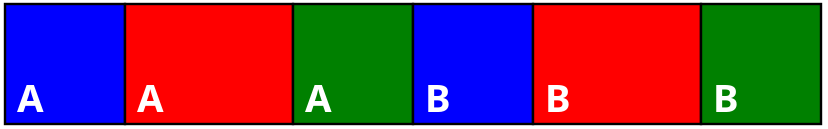
\includegraphics[width=\linewidth]{images/task_based_serial.png}
\caption{Task-based: una sola unità (esecuzione seriale).}
\label{fig:tb-1u}
\end{minipage}
\hfill
\begin{minipage}{0.48\textwidth}
\centering
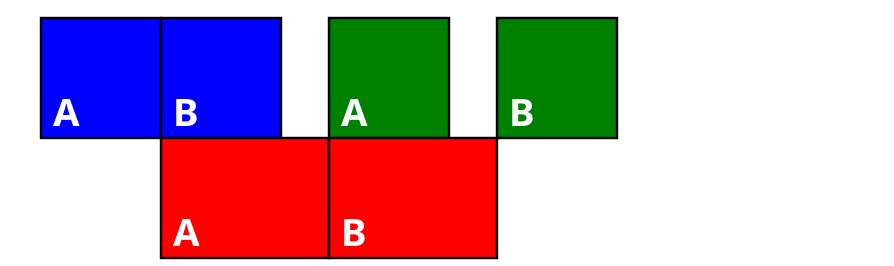
\includegraphics[width=\linewidth]{images/task_based_two_units_dependent.png}
\caption{Task-based: due unità, caso dipendente.}
\label{fig:tb-2u-dep}
\end{minipage}

\vspace{0.5cm}

\begin{minipage}{0.48\textwidth}
\centering
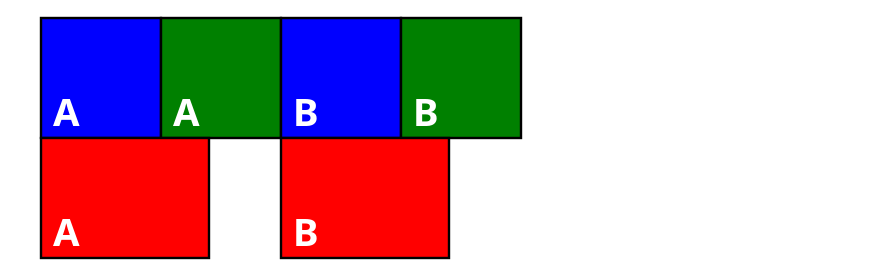
\includegraphics[width=\linewidth]{images/task_based_two_units_independent.png}
\caption{Task-based: due unità, caso indipendente.}
\label{fig:tb-2u-ind}
\end{minipage}
\hfill
\begin{minipage}{0.48\textwidth}
\centering
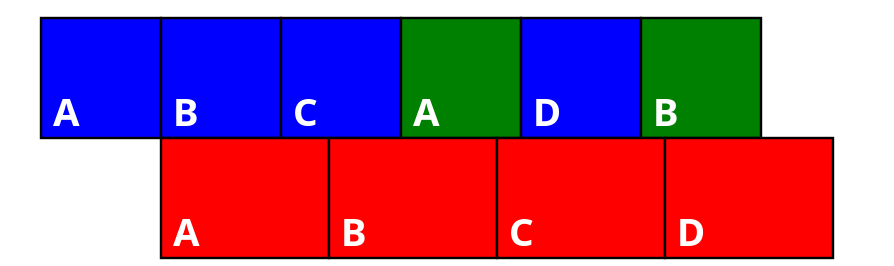
\includegraphics[width=\linewidth]{images/task_based_two_units_more_work_dependent.png}
\caption{Task-based: due unità, più lavoro, caso dipendente.}
\label{fig:tb-2u-dep-more}
\end{minipage}

\vspace{0.5cm}

\begin{minipage}{0.48\textwidth}
\centering
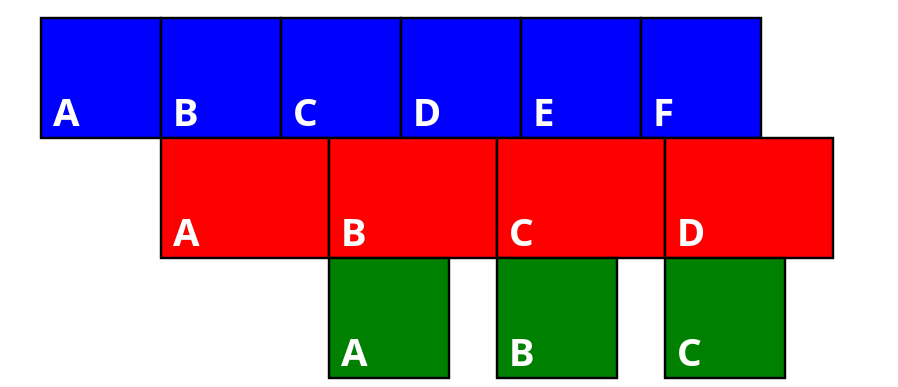
\includegraphics[width=\linewidth]{images/task_based_three_units_more_work_dependent.png}
\caption{Task-based: tre unità, più lavoro, caso dipendente.}
\label{fig:tb-3u-dep}
\end{minipage}
\hfill
\begin{minipage}{0.48\textwidth}
\centering
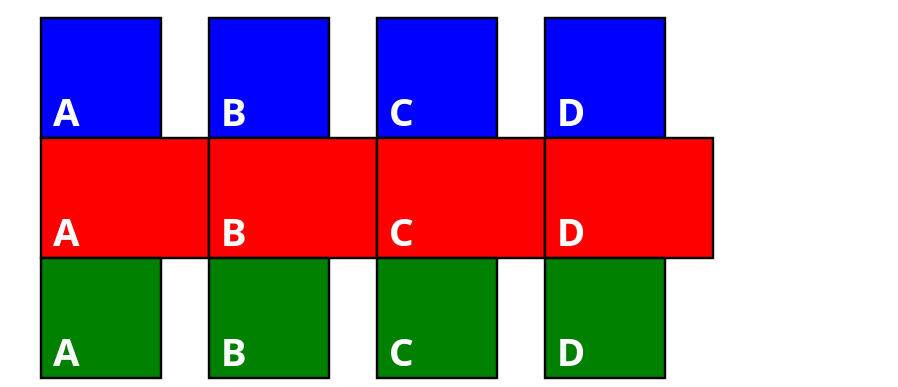
\includegraphics[width=\linewidth]{images/task_based_three_units_more_work_independent.png}
\caption{Task-based: tre unità, più lavoro, caso indipendente.}
\label{fig:tb-3u-ind}
\end{minipage}

\end{figure}

\subsection{Data-based parallelism}